\documentclass{standalone}
\usepackage{tikz}
\usepackage{verbatim}
\begin{document}
\pagestyle{empty}
  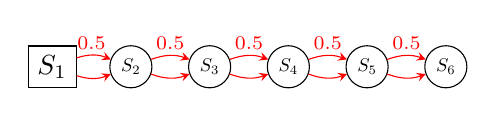
\begin{tikzpicture}
    \node[draw,rectangle] (l) at (-3, 0) {$S_1$};
    \node[draw,circle,scale=2/3] (a) at (-2, 0) {$S_2$};
    \node[draw,circle,scale=2/3] (b) at (-1, 0) {$S_3$};
    \node[draw,circle,scale=2/3] (c) at (+0, 0) {$S_4$};
    \node[draw,circle,scale=2/3] (d) at (+1, 0) {$S_5$};
    \node[draw,circle,scale=2/3] (e) at (+2, 0) {$S_6$};
    
    \path[-stealth] (a) edge[red,bend left=+20] (b);
    \path[-stealth] (a) edge[red,bend left=-20] (b);
    \node [red] at (-1.5, 0.3) {\scriptsize 0.5};
    
    \path[-stealth] (b) edge[red,bend left=+20] (c);
    \path[-stealth] (b) edge[red,bend left=-20] (c);
    \node [red] at (-.5, 0.3) {\scriptsize 0.5};
    
    \path[-stealth] (c) edge[red,bend left=+20] (d);
    \path[-stealth] (c) edge[red,bend left=-20] (d);
    \node [red] at (0.5, 0.3) {\scriptsize 0.5};
    
    \path[-stealth] (d) edge[red,bend left=+20] (e);
    \path[-stealth] (d) edge[red,bend left=-20] (e);
    \node [red] at (1.5, 0.3) {\scriptsize 0.5};
    
    \path[-stealth] (l) edge[red,bend left=+20] (a);
    \path[-stealth] (l) edge[red,bend left=-20] (a);
    \node [red] at (-2.5, 0.3) {\scriptsize 0.5};

  \end{tikzpicture}
\end{document}